\subsubsection{Encoder}
\label{sec:encoder}

A driver module for the encoder on the motor was part of the material to get started on this project. \cite{encoder_module}

\begin{figure}[H]
	\centering
	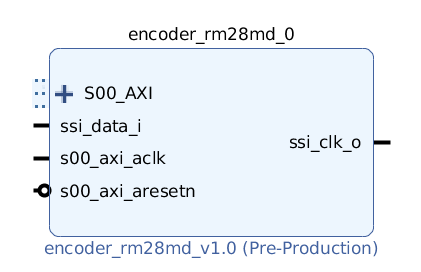
\includegraphics[width=0.4\textwidth]{pictures/software/encoder_module.png}
	\caption{The encoder driver module.}
	\label{fig:encoder_module}
\end{figure}
The driver module, as seen on figure \ref{fig:encoder_module}, supports an 8-bit encoder and takes care of handling the returned signal from the encoder itself. The module outputs the current rotor angle at a frequency determined by the PL clock and can be found with equation \ref{eq:encoder_frequency}.
\begin{equation}
f_{encoder} = \frac{f_{pl}}{6708} = \frac{125MHz}{6708} = 18.634kHz
\label{eq:encoder_frequency}
\end{equation}
The system runs at $10kHz$ which means the control loop will always have a new encoder angle at every cycle.


The encoder is a 8 bit encoder which means it has a resolution of $2^8 = 255$ steps per revolution. The motor has $4$ pole pairs which means the electric field inside the motor turns $4$ times each time the rotor turns $1$ time which means the resolution of the electric field angle is $1/4th$ of the mechanical rotor angle.
The two angles are both shown in figure \ref{fig:rotor_vs_electric_angle} where it can be seen that the electric angle moves 4 times faster than the rotor angle.

\begin{figure}[H]
	\centering
	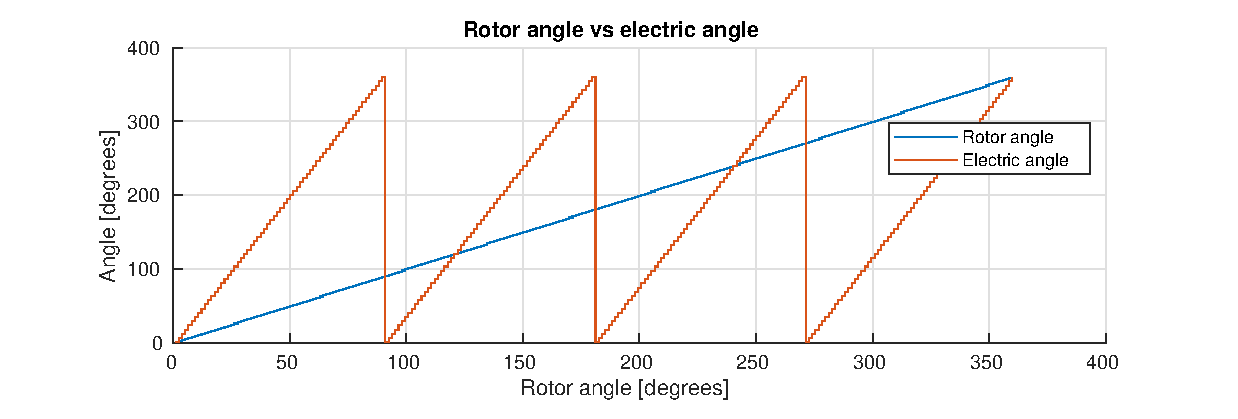
\includegraphics[width=1\textwidth]{pictures/software/rotor_vs_electric_angle.eps}
	\caption{Electric angle shown again the rotor angle.}
	\label{fig:rotor_vs_electric_angle}
\end{figure}

The resolution on the rotor angle and the electric angle can be calculated with equation \ref{eq:rotor_angle_error} and equation \ref{eq:electric_angle_error} respectfully. 

\begin{equation}
res_{rotor} = \frac{360^o}{2^8} = 1.412^o
\label{eq:rotor_angle_error}
\end{equation}

\begin{equation}
res_{electric} = \frac{360^o}{2^6} = 5.625^o
\label{eq:electric_angle_error}
\end{equation}




The rotor position is returned as an 8 bit value from the encoder module, and before the angle can be used in the control system it is first mapped from $0 \rightarrow 255$ to an actual angle going from $0^o \rightarrow 359^o$. The mapping is done with equation \ref{eq:angle_mapping}.
\begin{equation}
    angle = \frac{359}{255} \cdot position
    \label{eq:angle_mapping}
\end{equation}



\begin{lstlisting}[style=c, caption=Function to read an angle from the encoder. The angle is returned in degrees., label=code:encoder_angle_function]
f32 getRotorAngle(){
    u8 position = RM28MD_POSITION & 0x000000FF;     // Only the first byte is valid
    f32 angle   = 359/255 * position;       	      // Map position (0->255) to 
                                                    // angle (0->359)
    return angle;                                   // Return angle
}
\end{lstlisting}


\paragraph{Improve angle accuracy with linear interpolation}
\label{sec:linear_interpolation}
Low resolution and thereby big steps in the rotor angle results in uneven rotation of the motor especially at low speeds.
To improve the angle before it is used in the control the real angle is approximated with the use of linear interpolation. It is assumed that the rotor speed is approximately the same for each encoder value step. This assumption is not completely correct because it would mean the motor does not change speed. The rotor acceleration and deceleration is assumed slow enough compared to the encoder frequency to not result in big errors.


The formula for linear interpolation \cite{lin_interpol} can be seen in equation \ref{eq:linear_interpolation1}. 

\begin{equation}
    y = \Big( \frac{y_2-y_1}{x_2-x_1} \Big)(x-x_1)+y_1
    \label{eq:linear_interpolation1}
\end{equation}
Figure \ref{fig:angle_interpolation1} shows the scenario where the real angle, at point $p_2$, can be found from the measured angle, $p_1$, if $x_1$,$x_2$,$y_1$ and $y_2$ are known.
The equation can be converted to fit the system by setting the two $y$ values equal to the amount of change between the current and last step $\Delta a = y_2 - y_1$ and setting the $x$ values to be the step width $x_{step} = x_2 - x_1$. Assuming that the speed is approximately the same for the current step as it was on the last. Which results in equation \ref{eq:linear_interpolation2}.

\begin{equation}
    y =  \frac{\Delta a}{x_{step}} \Delta x+y_1
    \label{eq:linear_interpolation2}
\end{equation}

\begin{figure}[H]
	\centering
	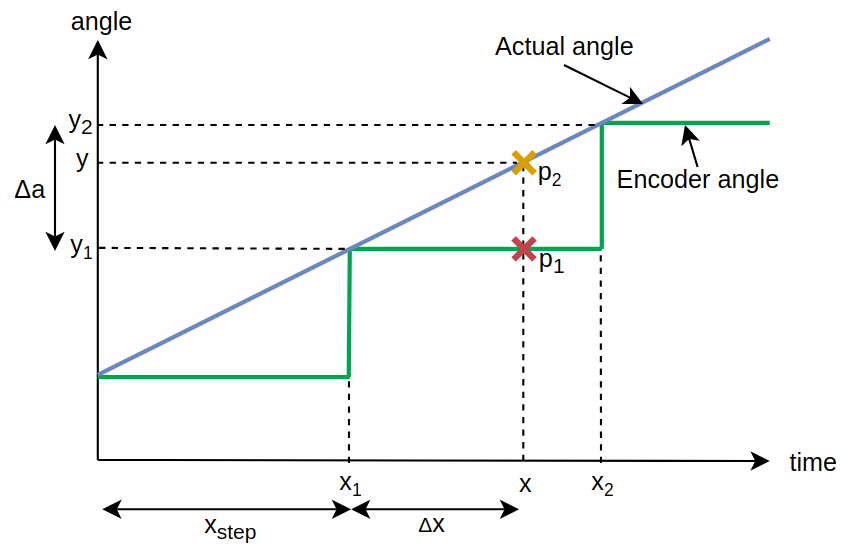
\includegraphics[width=0.8\textwidth]{pictures/software/angle_interpolation1.png}
	\caption{Ideal linear interpolation.}
	\label{fig:angle_interpolation1}
\end{figure}

The x-axis is discrete time and will be kept track of in relation to the number of samples passing and therefore $x$ will be denoted $n$. To know how fast the encoder values change over time this frequency is calculated with equation \ref{eq:encoder_step_frequency}.

\begin{equation}
    f = \frac{v_{[^o/s]}}{res_{rotor}} = 5000 [RPM] \cdot 6 \cdot \frac{360^o}{2^8} = 42188Hz
    \label{eq:encoder_step_frequency}
\end{equation}

The frequency is more than four times faster than the sampling frequency which means that not every encode value step will be sampled. The interpolation will only work if the is at least 2 samples on a step. To find the maximum speed where the interpolation works it is found where the encoder step frequency is lower than $10kHz$.

\begin{subequations}
	\begin{align}
    	\begin{split}
        	10kHz > v_{RPM}\cdot 6 \cdot res_{rotor}
    	\end{split} \\ 
    	\begin{split}
        	v_{RPM} < \frac{10kHz}{6 \cdot res_{rotor}}
    	\end{split} \\
    	\begin{split}
        	v_{RPM} < \frac{10kHz \cdot 2^8}{6 \cdot 360}
    	\end{split} \\
    	\begin{split}
        	v_{RPM} < 1185 RPM
    	\end{split} 
	\end{align}
\end{subequations}

When the rotor speed is less than $1185RPM$ the system will sample at least $1$ time per encoder step.

Equation \ref{eq:linear_interpolation2} can be further changed to fit the system.
\begin{equation}
    a_{i} = \frac{\Delta a}{n_{step}} n_{samples} + a
    \label{eq:linear_interpolation3}
\end{equation}
% Where $n_{step}$ is the number of samples on the last step and $n_{samples}$ is the amount of samples before the current sample on the same step as can be seen in figure \ref{fig:angle_interpolation2}.
Where $a_{i}$ is the interpolated angle, $n_{step}$ is the number of samples on the last step, $n_{samples}$ is the number of samples before the current sample on the current step, $a$ is the angle received from the encoder, as can be seen in figure \ref{fig:angle_interpolation2}.

\begin{figure}[H]
	\centering
	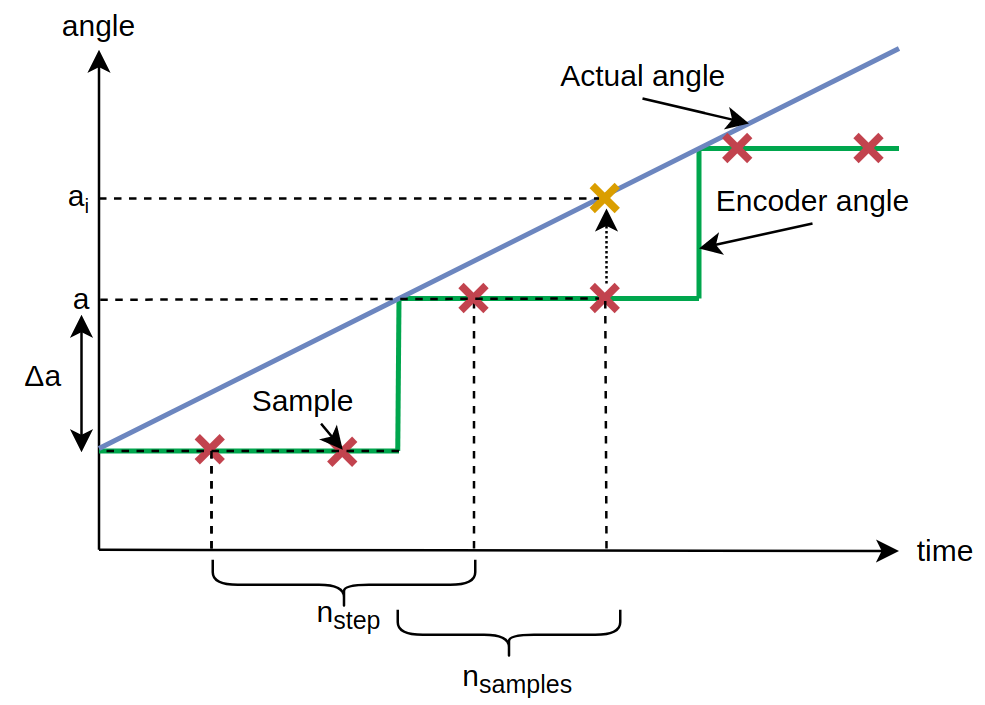
\includegraphics[width=0.8\textwidth]{pictures/software/angle_interpolation2.png}
	\caption{Practical version of linear interpolation.}
	\label{fig:angle_interpolation2}
\end{figure}






% The motor maximum speed is $5000RPM$ so the interpolation should be able to handle steps being skipped.

Equation \ref{eq:linear_interpolation3} can be rewritten to have the two counters as the fraction resulting in equation \ref{eq:linear_interpolation}.
\begin{equation}
a_{i} =  \frac{n_{samples}}{n_{step}} \Delta a  + a
\label{eq:linear_interpolation}
\end{equation}

$n_{samples}$ are a count of the number of samples on the current step. The counter starts at $0$ which means $n_{samples} \leq n_{steps}$ if the speed is approximately the same for the current and last encoder step.

\begin{equation}
	0 \leq	\Big(\frac{n_{samples}}{n_{step}} \Big) \leq 1
\end{equation}
Which means that the output of the interpolation is limited to
\begin{equation}
	 a \leq a_i \leq (a + \Delta a)
\end{equation}


The finished interpolation algorithm can be seen in the code snippet \ref{code:interpolation_algorithm} below. 

Every time the function is called a counter, \textit{time}, is incremented and this counter keeps track of the time.

Line $5$ to $8$ handle the first time the interpolation is used and it updates the variable $t\textunderscore 1$ which is the time of the left edge of the counter $n_{step}$. 

Line $10$ to $15$ handles the interpolation until the right edge of $n_{step}$ is updated, this is done with the variable $t\textunderscore 2$. For both the edges the value from the encoder is saved from the encoder to handle the step size in case one or more steps are skipped.

Line $17$ to $29$ handle the actual running algorithm. The sample counter is incremented. If a new step is reached the left edge is set the the last right edge, $t\textunderscore 1 = t\textunderscore 2$, and the new right edge is updated, $t\textunderscore 2 = angle$.

The step width is calculated as well as the step size which results in all the variable ready to calculate the interpolated angle on line $28$ as per equation \ref{eq:linear_interpolation}.

\begin{lstlisting}[style=c, caption=Interpolation algorithm implemented on the embedded system., label=code:interpolation_algorithm]
f32 interpolateAngle(f32 angle){
	time++;								                 // Keep track of time
	f32 angleInterpolated = angle;		     // Default value of angle
	/* First time used */
	if(t1 == 0){
		t1 = time;						               // Update time of t1
		t1v = angle;					               // Update angle of t1
	}
	/* If t2 has not been updated for the first time yet */
	if(t2 == 0){
		if(angle != t1v){				             // Check if first step happens
			t2 = time;					               // If so update time for t2
			t2v = angle;				               // Update angle of t2
		}
	}
	/* For all other steps than the first two */
	if(t1 != 0 && t2 != 0){				         // Do the actual interpolation
		nSamples++;						               // Keep track of samples on current step
		if(angle != t2v){				             // If new step happens
			t1 = t2;					                 // Move t2 to t1
			t1v = t2v;					               // Update value of t1
			t2 = time;					               // Update t2 to current time
			t2v = angle;				               // Update value of t2 to current angle
			nSamples = 0;				               // Reset number of samples on step
		}
 		u32 nStep = t2 - t1;				         // Get time on last step (approximation)
		f32 angleStep = t2v-t1v;	           // Get angle step
		angleInterpolated = nSamples/nStep * angleStep + angle; // Calculate new angle
	}
	return angleInterpolated;			         // Return new angle
}
\end{lstlisting}

To measure the improvement of the interpolated angle compared to the encoder angle a sweep of the motor speed from 1RPM to 5000RPM has been performed. The sweep was done with the algorithm implemented in Matlab. The results are shown on figure \ref{fig:interpolation_error}. The interpolated error is smaller for speeds less than $1185RPM$ otherwise the interpolation error is the same as the general error.


\begin{figure}[H]
	\centering
	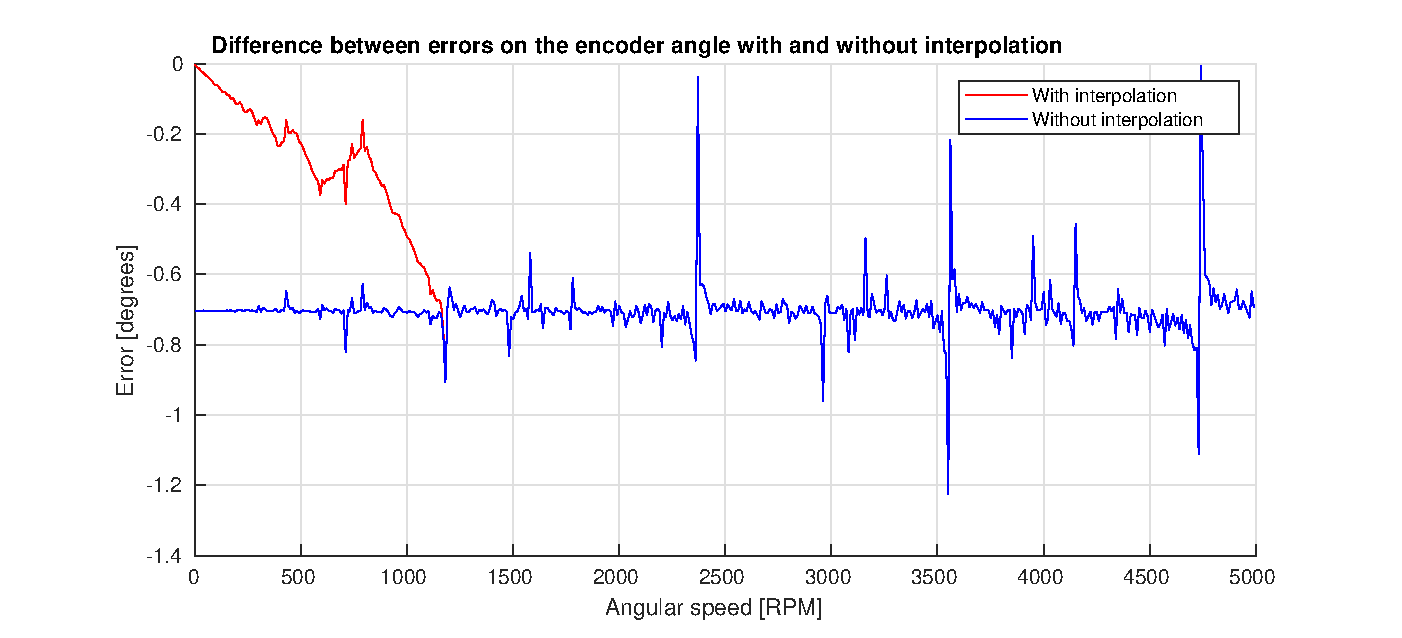
\includegraphics[width=1\textwidth]{pictures/software/interpolation_error.eps}
	\caption{Frequency sweep of angular error with and without linear interpolation.}
	\label{fig:interpolation_error}
\end{figure}


\subsubsection*{Conclusion}
The angle interpolation works to limit the encoder angle error for speeds under $1185RPM$ but speeds over $1185RPM$ the interpolation just follows the normal encoder angle error.